\chapter{Synthedemic Modelling}
\label{ch:multi}
The classic epidemic model brings to mind images of a single curve
with a single peak. When measuring the spread of a single infectious
disease within a closed population, this is often a realistic
characterisation. For example, the number of people in London infected
with a new strain of flu virus might resemble this curve. 

Recent work has highlighted the limitations of the single epidemic
based approach in characterising certain epidemic phenomena, particulary with
regards to viral internet trends.\cite{marily2013, marily2014} A
recent adaptation of the field of \emph{synepidemiology} termed
\emph{synthemics} has been proposed as a potential avenue of further
research. The key challenges of the synthedemic modelling procedure are to
identify the number of underlying epidemics, to identify when these
sub epidemics start, and to identify the type of epidemic model that
best describes each sub epidemic. Furthermore, as the number of
included sub epidemics increases, so to do the number of parameters to
be optimised the corresponding parameter search space. 

In this section we discuss an implementation that aims to address these challenges,
and the particular problems and solutions that arise during the course
of the project.


\section{Identifying Sub Epidemic Start Time}
In the single epidemic fitting framework, it is assumed that there is
only one epidemic in the dataset, and that it can be considered to
have started right from the start of the data, $t_0$. However, when
considering multiple epidemics simultaneously, it is not possible to
make this assumption, as multiple sub epidemics might start and finish during
the iterative fitting procedure. Furthermore, when multiple epidemics
are progressing simultaneously, it might not be possible to detect the
start of a new epidemic until it is well underway. The start time of
the epidemic therefore might (and probably will not) match the
detection time. The first step in developing a
synthedemic model fitting framework is therefore to implement a means
to detect and record epidemic start times, and to consider how these
start times will be included in the optimisation procedure.

\subsection{Epidemic Detection}

\subsection{Optimising Epidemic Start Times}
Once an epidemic outbreak has been detected, the next challenge is to
find the actual start time of the epidemic. Simply using the detection
time of the sub epidemic as the actual start time is unsatisfactory,
as it assumes that the detection procedure will pick up a new outbreak
as soon as it starts. Some sub epidemics will be hidden within larger
outbreaks and may not be detected until well into their course. 

An initial naive approach to finding the start time of each sub
epidemic might be to consider each possible combination of epidemic
start times. If we consider every possible start time, this would
result in \emph{n}
optimisations for a single epidemic, where \emph{n} is the number of
data points currently available. As soon as multiple epidemics are
considered simultaneously, this quickly becomes infeasible as the
complexity increases with the number of sub epidemics. An heuristic adaption to this is to only consider a subset of start
time combinations. For example, we can consider only the start times
within a window of the detection time, and assume that the ordering of
start times does not matter. This results in \emph{tCn} combinations
of start times, where \emph{t} is the number of time points under
consideration, and \emph{n} is the number of epidemics to be
fit. 

Although such heuristics  might provide a
conceptually simple optimisation approach, they avoid the problem of
including $t_0$ in the optimisation procedure directly. Doing should
allows for the start time of each sub epidemic to be found
precisely. Furthermore, doing so allows us to consider the start time
as a continuous variable, making the model fit much more accurate. We
therefore chose to initially include $t_0$ as an unknown parameter in
the optimisation procedure. Giving the Nelder Mead algorithm a
completely random time as a seed value risks producing an extremely
high initial SSE value. We therefore use the detection time minus a
small value (to account for delayed detection) of the epidemic
as the seed value for the optimisation procedure. 

\section{Initial Approach}
The initial approach aims to iterate over a set of epidemic data,
where it is not assumed that there is an ongoing epidemic from the
start. We include the transition parameters, beta and gamma, as well
as S0 and t0 in the optimisation procedure. As in the single fitting
framework, at each time point we produce random seed values and choose
the best run from ten independent as the best fitting model. T0 is
seeded as the detection time of the epidemic. We first fit the
currently known \emph{k} epidemics, and then consider the addition of
an epidemic when the model fit has deteriorated sufficiently and
the latest residual is a certain number of standard deviations away
from the previous residuals' mean. By only adding an additional
epidemic when the model fit has deteriorated sufficiently, we avoid
needlessly overfitting the data when an outlying data point might
falsly suggest the start of a new epidemic.

We initially consider only SIR models, which result in a combined
parameter set of $(\beta^{(k)},\gamma^{(k)},\S_{0}^{(k)},t_0^{(k)})$ to
be optimised. One risk of only considering the addition of epidemics
is that we risk overfitting the data. To avoid this, we also consider the removal of a
sub epidemic at each time point. This is done by removing each sub
epidemic from the current set in turn and reoptimising the remaining
model. If this fit of $k-1$ epidemics is sufficient, we
permanently remove the epidemic from the list.

\subsection{Initial Testing}
The multiple epidemic fitting framework was firstly tested using
synthetic data generated by the \emph{GillespieSSA} algorithm in R. To
simulate multiple overlapping epidemics, we run \emph{GillespieSSA}
for each sub epidemic and offset the values by the desired $t_0$;
adding the infected values of each sub epidemic on the corresponding
time points. Two \emph{SIR} models were combined with the following
parameters:

$\beta^1=0.001, \gamma^1 = 0.01, S_0 = 500, t_0 = 10$\\
$\beta^1=0.0008, \gamma^1 = 0.008, S_0 = 800, t_0 = 30$

The initial implementation detected the start of the first epidemic at
$t = 14$, and proceeded to accurately fit the the epidemic. At around
$t = 30$, the second epidemic was detected and added to the
optimisation procedure. The R Square value for the model fit to the
currently known values remains high throughout the fitting procedure
at over 0.99, though it does occasionally fall to around 0.95. This is
likely due to poor initial seed values.

\begin{centering}
\begin{figure}[h!]
  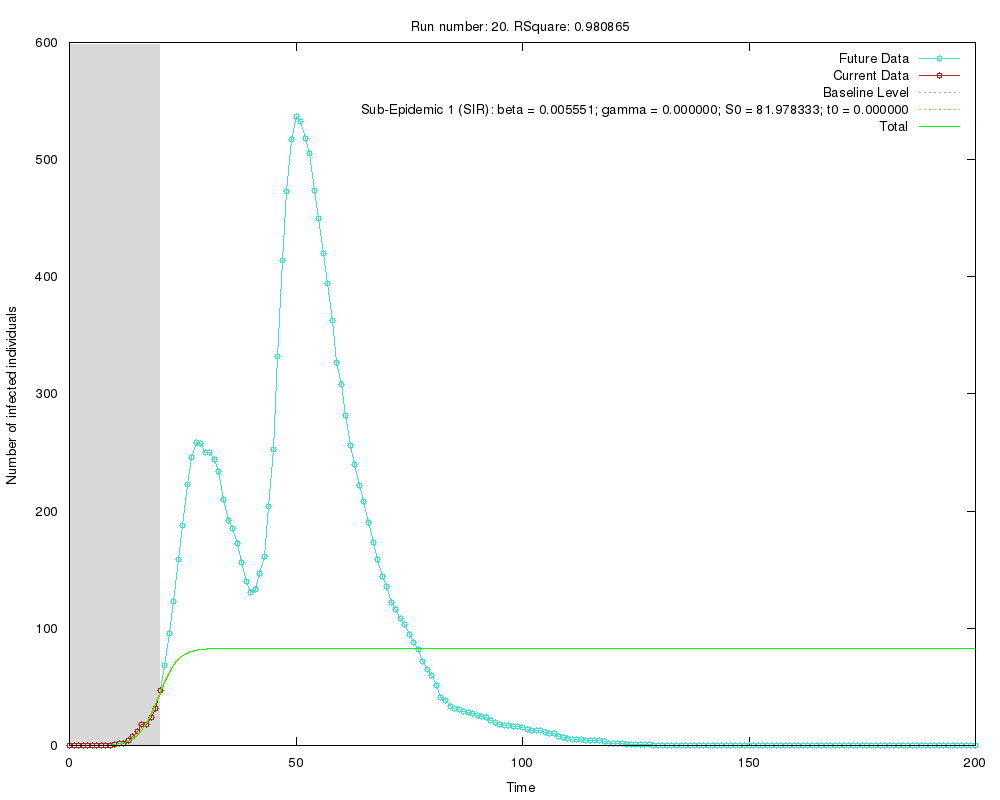
\includegraphics[width=8cm]{images/multi/sirsir1.png}
  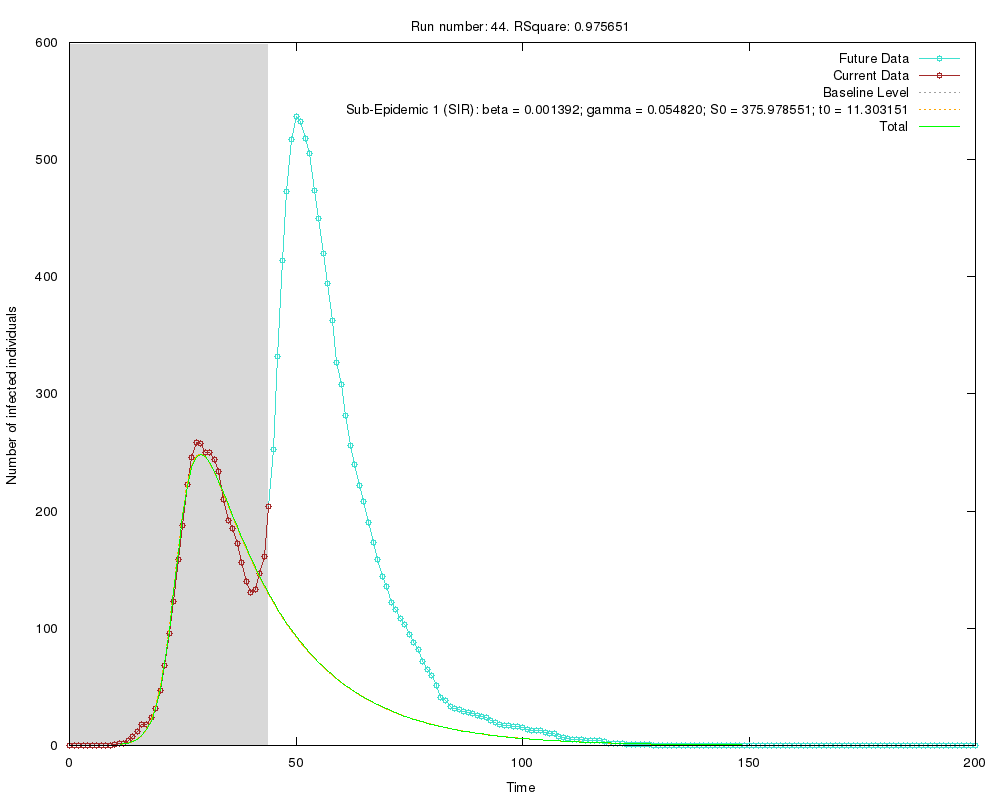
\includegraphics[width=8cm]{images/multi/sirsir2.png}
  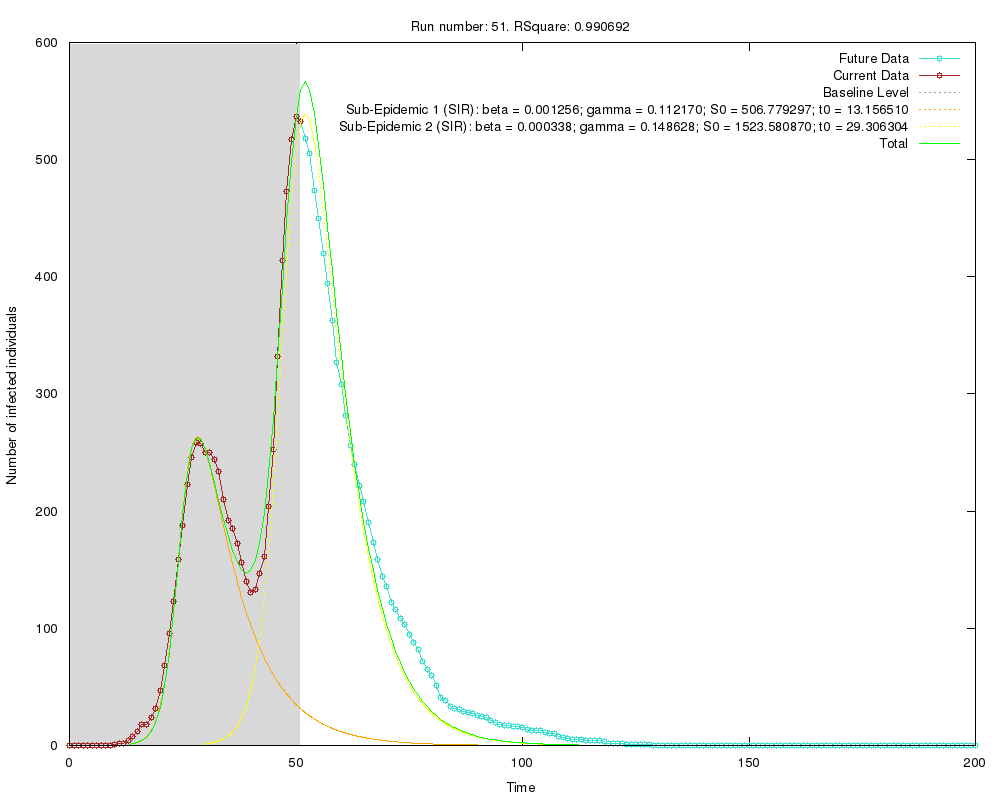
\includegraphics[width=8cm]{images/multi/sirsir3.png}
  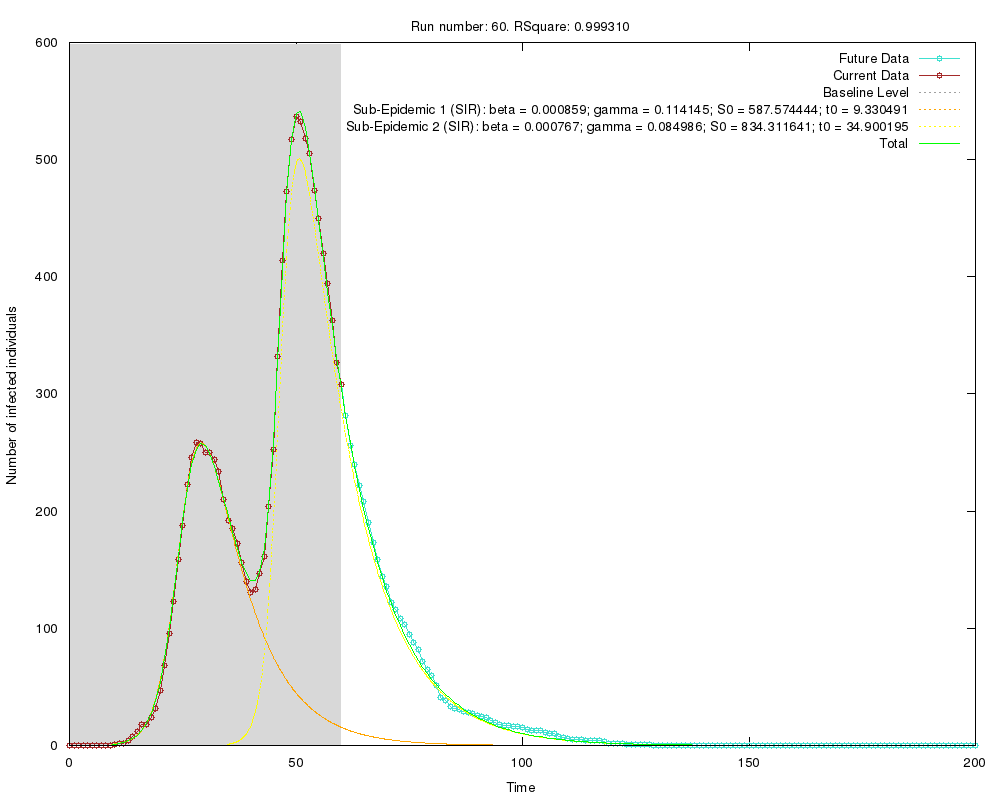
\includegraphics[width=8cm]{images/multi/sirsir4.png}
  \caption{Multiple epidemic fitting procedure on two overlapping SIR models}
\label{fig:sirsir1}
  \end{figure}
\end{centering}




\subsection{Parameter Transformations and Bounding}
As discussed in section SECTION, it is often desirable to transform the
model parameters into log space. Another potential transformation that may be applied is through the
use of the \emph{logistic} function. Originally studied in the context
of population growth, maps the parameter search space from between $0$ and $1$
to between $-\infty$ and $+\infty$. The function is
defined as:
\begin{equation}
logistic(x)=\frac{1}{1+e^{-x}}
\end{equation}
The inverse of the logistic function, the \emph{logit} function, can
therefore be used to map the search space of a parameter, \emph{p},
from between $-\infty$ and $+\infty$ to between $0$ and $1$. The logit
function is defined as:
\begin{equation}
logit(p) = log(\frac{p}{1-p})
\end{equation}
The logit function can be modifed to transform the search space from
between $0$ and $1$ to one between $0$ and $max$ as follows:
\begin{equation}
newLogit(x) = \frac{max}{1+e^{-x}}
\end{equation}
with the inverse defined as:
\begin{equation}
newLogistic(x)=log(\frac{x}{max-x})
\end{equation}

 The logic behind this modification can be expanded further to use the logistic function to provide lower bounds as well as upper bounds. As
$x\rightarrow +\infty$, $logit(x)\rightarrow 1$. Similarly, as
$x\rightarrow-\infty$, $logit(x)\rightarrow 0$. We can therefore modify
the logistic function as follows:
\begin{equation}
f(x) = \frac{x_{max}-x_{min}}{1+e^{-x}} + x_{min}
\end{equation}.

We can see that as $x\rightarrow +\infty$, $f(x)\rightarrow x_{max}$,
and as $x\rightarrow -\infty$, $f(x)\rightarrow x_{min}$. By limiting
the parameter search space to a predetermined range of expected
values, we ensure that the optimisation procedure does not get stuck
in a local minimum far away from the actual parameter values. However,
doing so requires us to make assumptions regarding where the real
parameter values might lie. Whilst a good model fit might be produced
within a provided range of parameter values, this fit might be sub
optimal compared to the model produced from a set of entirely
unexpected parameters. 

An alternative, simple approach to bounding parameter values in the
optimisation procedure is to modify the results returned by the
objective function. As the Nelder Mead algorithm transforms parameter
values with the aim of minimising the objective function, we can
direct the parameter search by ensuring that the objective function
returns high values when venturing into an undesirable parameter
space. For example, we can include a simple check of each parameter
with each call of the objective function; returning a high SSE value
if the parameter is outside our desired range. This method was
implemented initially; however, it appeared to result in the Nelder
Mead algorithm returning nonsense values more frequently as it failed
to identify any local minima. This is due to the fact that the
optimisation surface becomes much less smooth, as each check outside
of the specified bounds results in a sudden spike in function value.  


\section{Implementation Revision with Parameter Bounding}


\section{Final Implementation}


\section{Real Data Testing}
